\documentclass[10pt]{beamer}

\usetheme[progressbar=frametitle]{metropolis}
\usepackage{appendixnumberbeamer}

\usepackage{booktabs}

\usepackage{graphicx}
\usepackage{subfig}
\usepackage{multirow}
\usepackage{multicol}
%\usepackage[brazilian]{babel}
\usepackage[utf8]{inputenc}
\usepackage[T1]{fontenc}

\usepackage[scale=2]{ccicons}

\usepackage{pgfplots}
\usepgfplotslibrary{dateplot}

\usepackage{xspace}
\newcommand{\themename}{\textbf{\textsc{metropolis}}\xspace}

\title{ncRNA classification using complex networks topological measures}
\subtitle{Programa de P\'os Gradua\c{c}\~ao Associado em Bioinform\'atica UFPR/UTFPR-CP}
\date{\the\year}
\author{Matheus Henrique Pimenta-Zanon and Fabrício Martins Lopes}
\institute{Universidade Federal do Paraná and Universidade Federal do Paran\'a - Corn\'elio Proc\'opio}
\titlegraphic{\hfill
\includegraphics[height=1cm]{fig/logo.png}}

\begin{document}

\maketitle

\begin{frame}{Table of contents}
  \setbeamertemplate{section in toc}[sections numbered]
  \tableofcontents%[hideallsubsections]
\end{frame}

\section[Introduction]{Introduction}

\begin{frame}[fragile]{RNA}

\begin{itemize}
    \item RNA sequences can play various functional roles in the organism;
    \pause
    \item In general, they can be classified as coding (mRNA) and non-coding (ncRNA);
    \pause
    \begin{itemize}
        \item The mRNAs are translated in proteins necessary for cellular functions;
        \pause
        \item The ncRNA have several families and their role are still not fully understood;
    \end{itemize}
\end{itemize}
\end{frame}

\begin{frame}{ncRNA}
    The role of some ncRNA is the over participation in complex human diseases, such as cancer, Alzheimer’s disease, and cardiovascular diseases \cite{Esteller2011, Shi2013}.
\end{frame}

\begin{frame}{Next-generation sequencing (NGS)}
    The Next-generation sequencing (NGS), in particular the RNA-seq method, generates reads and assembling transcripts of diverse unclassified RNA.
\end{frame}


\subsection{Objectives}

\begin{frame}[fragile]{Objectives}
\begin{itemize}
    \item Propose an extension of the feature extraction method, named BASiNET \cite{ito_basinetbiological_2018-1};
    \pause
    \item Fewer thresholds are used to order to classify different RNA classes, considering four small non-coding RNA (small ncRNA) families (tRNA, IRES, miRNA, and 5SrRNA).
\end{itemize}

\end{frame}

\section{Materials and Methods}

\subsection{Materials}

\begin{frame}{Materials}
    The Rfam9 dataset \cite{Gardner2010} was used to provide the ncRNA sequences input to the proposed method. 
\end{frame}

\subsection{Methods}

\begin{frame}{Methods}
\begin{figure}[!ht]
	\centering
	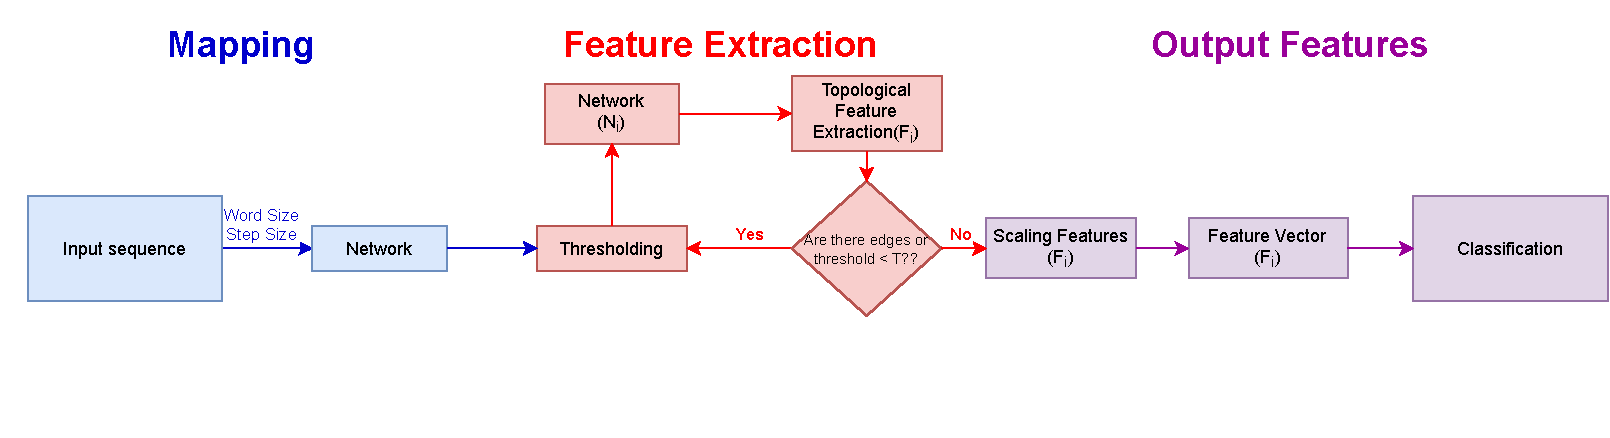
\includegraphics[scale=0.4]{fig/overview.pdf}
	\caption{Overview of the BASiNET method.}
	\label{fig:overview}
\end{figure}  
\end{frame}

\begin{frame}{Methods}
\begin{figure}[!ht]
	\centering
	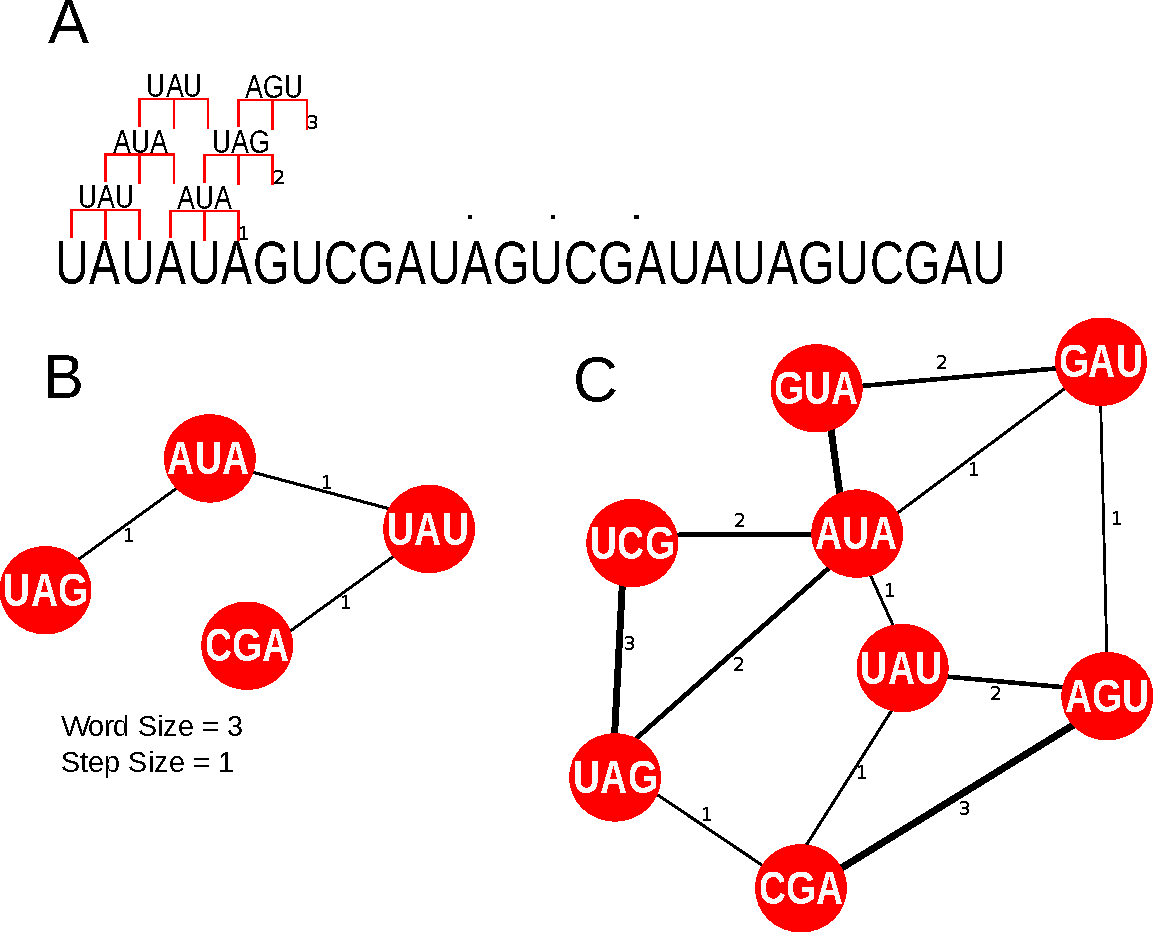
\includegraphics[scale=0.4]{fig/mapping.pdf}
	\caption{Mapping step of the BASiNET method.}
	\label{fig:overview}
\end{figure}  
\end{frame}

\section{Preliminary results}

\begin{frame}{Preliminary results}
Using fewer thresholds values the accuracy maintains suitable results, using the Decision Tree classifier to reach 88\% accuracy in a small dataset.

\pause

\begin{figure}[!ht]
	\centering
	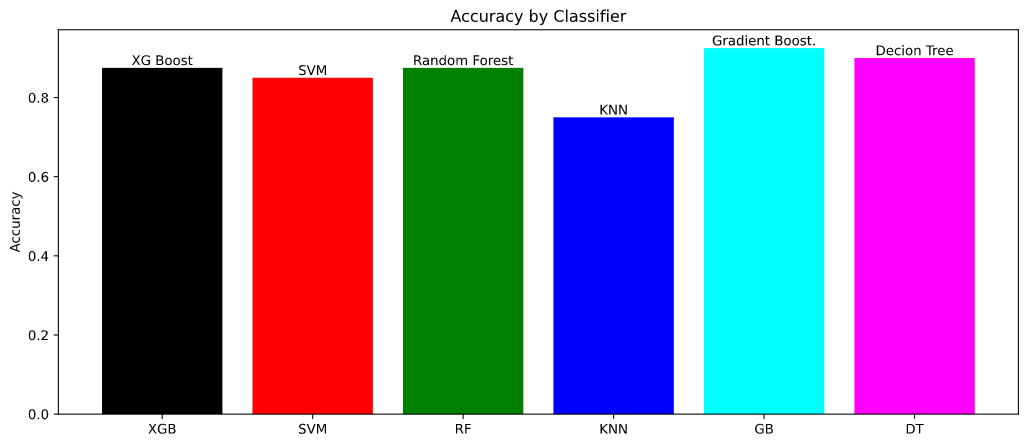
\includegraphics[scale=0.3]{fig/barplot.png}
	\caption{The  highest  average  accuracy  of  the  10-fold  cross  validation  achieved  from  the adopted threshold and classifiers when considering the features extracted by BASiNET.}
	\label{fig:overview}
\end{figure}  
    
\end{frame}

\section{Conclusion}

\begin{frame}{Conclusion}
Using fewer thresholds values the accuracy maintains suitable results;

\pause

The capacity to classify different ncRNA sequences, which is not shown in the first BASiNET version.

\end{frame}

{\setbeamercolor{palette primary}{fg=black, bg=yellow}
\begin{frame}[standout]
  Thank you!
  
  \pause
  
  \footnotesize{We would like to thank the Coordenação de Aperfeiçoamento de Pessoal de Nível Superior (CAPES) for funding this work.}
\end{frame}
}

\begin{frame}[allowframebreaks]{References}

  \bibliography{reflatex}
  \bibliographystyle{abbrv}

\end{frame}

\end{document}
